\subsection{Pump beam profile}
\label{sec:comsol:beamprofile}

For the heat source $Q$
in (\ref{eq:heateq})
we assume
the pump beam
is incident antiparallel to the $z$-axis
(here referred to as from the top),
and of Gaussian profile.
In this orientation the heat source
associated with
each layer $j$ of the structure is given as
\cite{Kemp2008}
\begin{equation}
Q_j = \frac{2P}{\pi w^2} \eta_j\alpha_j \e^\frac{-2r^2}{w^2} \e^{-\alpha_j(z_{0j}-z)} \e^{-\sum_{i<j}\alpha_i t_i}.
\label{eq:heatsrc}
\end{equation}
This representation counts the layers
from the top down --
the sum $\sum_{i<j}$ includes the layers on top
and ignores those below the layer of interest
(in that case $j$).
A derivation,
as well as a more in-depth explanation
what the different parameters stand for,
is given in
appendix~\ref{app:comsol_deriv:Q}.

Equation (\ref{eq:heatsrc})
describes a Gaussian pump profile
by design.
In reality, however,
the pump profile is most likely not Gaussian.
In fact,
the pump spot imaged from a multimode fiber
resembles a flat-top
(also known as top-hat)
distribution \cite{Tropper2006},
or at least a super-Gaussian
\cite{Chernikov2010,Heinen2012el}.
Figure~\ref{img:visuallize_sGauss}
illustrates the difference in beam shape
of these mentioned three types.

In order to incorporate
a flat-top pump profile,
we have to replace the Gaussian part
in (\ref{eq:heatsrc}) \cite{Kemp2005}:
\begin{equation}
2\e^\frac{-2r^2}{w^2} \to
\left\{
\begin{matrix}
1 & r\leq w \\
0 & r>w.\\
\end{matrix}
\right.
\label{eq:replflattop}
\end{equation}
This can easily be verified as the renormalization has to match,
\begin{equation}
\frac{2}{w^2} \int\limits_0^\infty r \d r \e^\frac{-2r^2}{w^2}
= \frac{1}{w^2} \int\limits_0^w r \d r = \frac{1}{2}.
\label{eq:heatsrc_renorm}
\end{equation}

A super-Gaussian is of the form \cite{Chernikov2010}
\begin{equation}
f(x) \propto \e^{-|\frac{x}{w}|^\beta}.
\label{eq:super-gauss}
\end{equation}
The Gaussian profile (\ref{eq:gaussE})
corresponds to the special case $\beta=2$,
and the flat-top distribution to $\beta=\infty$.
Parameter $w$ corresponds
to the $\e^{-2}$ radius
\begin{equation}
w = \frac{\mathrm{FWHM}}{2(\frac{1}{2}\log2)^{1/\beta}}.
\end{equation}
This definition of $w$ is necessary
in order to be compatible
with the definition
of the flat-top distribution
already known in literature
\cite{Kemp2005}.
However,
in \cite{Heinen2012el}
they measured the profile
of their super-Gaussian pump,
and decided to report
the FWHM
as spot diameter.

Before we can incorporate a super-Gaussian,
we have to numerically find the normalization factor
\begin{equation}
a_p = \frac{2}{w^2} \int\limits_0^\infty r \d r \e^{-2|\frac{r}{w}|^\beta}.
\label{eq:super-gauss-scaling}
\end{equation}
Analogously to (\ref{eq:replflattop}),
for a super-Gaussian profile
we replace in (\ref{eq:heatsrc})
\begin{equation}
2\e^\frac{-2r^2}{w^2} \to \frac{1}{a_p}\e^{-2|\frac{r}{w}|^\beta}.
\label{eq:replsupergauss}
\end{equation}
Four examples for the normalization factor,
rounded to four digits, are
$a_{2}=0.5$,
$a_{3}=0.5687$,
$a_{4}=0.6267$,
and $a_\infty=0.5$.
See also
the analytic results in (\ref{eq:heatsrc_renorm}),
and Fig.~\ref{img:visuallize_sGauss}.

\begin{figure}
\centering
\subfigure{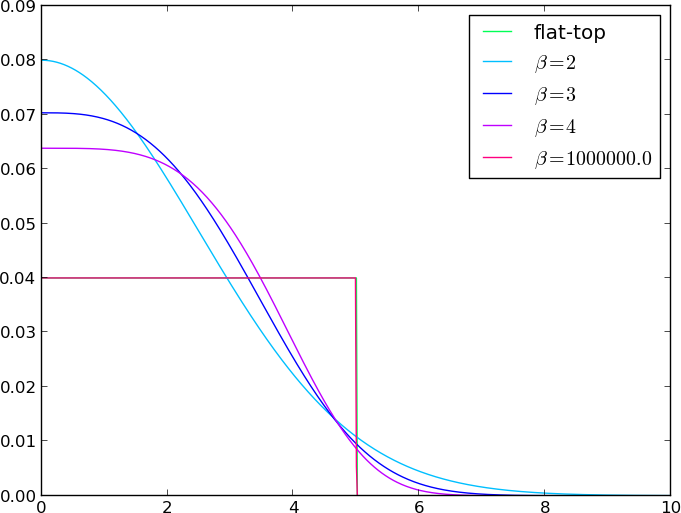
\includegraphics[width=7cm]{img/visuallize_super-Gauss_f2.png}}
\subfigure{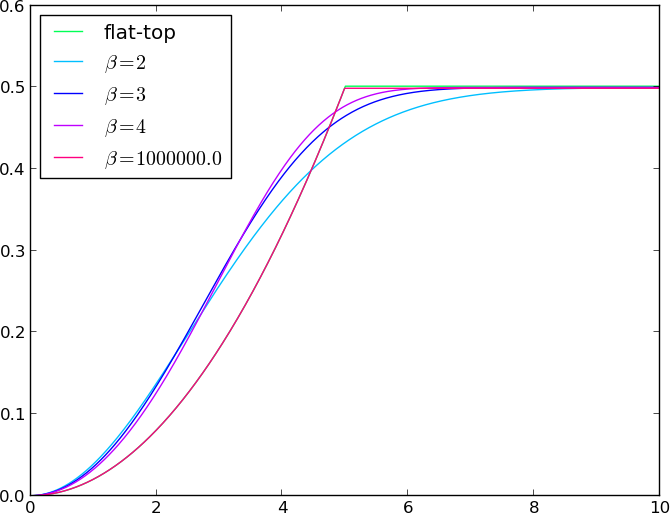
\includegraphics[width=7cm]{img/visuallize_super-Gauss_f2int.png}}
\caption{A super-Gaussian of the form
$f^2(x) \propto \e^{-2|x/w|^\beta}$
\cite{Chernikov2010}
describes an intermediate shape
between a regular Gaussian with $\beta=2$
and flat-top with $\beta=\infty$.
Left,
we see the squared shapes
of super-Gaussians $f^2(x)$ with $w=5$
for different values of $\beta$,
including flat-top as a point of reference.
The normalization is chosen such that
the over all integral corresponds to $0.5$;
from (\ref{eq:heatsrc_renorm}).
This is demonstrated in the plot to the right.}
\label{img:visuallize_sGauss}
\end{figure}